\documentclass{article}

\usepackage{fancyhdr}
\usepackage{extramarks}
\usepackage{amsmath}
\usepackage{amsthm}
\usepackage{amsfonts}
\usepackage{tikz}
\usepackage{placeins}
\usepackage{float}
\usepackage{url}
\usepackage[utf8]{inputenc}
\usepackage{tabularx}
\usepackage{booktabs}
\usepackage[plain]{algorithm}
\usepackage{algpseudocode}
\usepackage{listings}
\usepackage{xcolor}
\usepackage{graphicx}
\usepackage{subcaption}
\usepackage{hyperref}

\graphicspath{{images/}}

% Code style
\definecolor{codegreen}{rgb}{0,0.6,0}
\definecolor{codegray}{rgb}{0.5,0.5,0.5}
\definecolor{codepurple}{rgb}{0.58,0,0.82}
\definecolor{backcolour}{rgb}{0.95,0.95,0.92}
\lstdefinestyle{mystyle}{
    backgroundcolor=\color{backcolour},
    commentstyle=\color{codegreen},
    keywordstyle=\color{magenta},
    numberstyle=\tiny\color{codegray},
    stringstyle=\color{codepurple},
    basicstyle=\ttfamily\footnotesize,
    breakatwhitespace=false,
    breaklines=true,
    captionpos=b,
    keepspaces=true,
    numbers=left,
    numbersep=5pt,
    showspaces=false,
    showstringspaces=false,
    showtabs=false,
    tabsize=4
}
\lstset{style=mystyle}

\usetikzlibrary{automata,positioning}

% Page layout
\topmargin=-0.45in
\evensidemargin=0in
\oddsidemargin=0in
\textwidth=6.5in
\textheight=9.0in
\headsep=0.25in
\linespread{1.1}

\pagestyle{fancy}
\lhead{\hmwkAuthorName}
\chead{\hmwkClass\ : \hmwkTitle}
\rhead{\firstxmark}
\lfoot{\lastxmark}
\cfoot{\thepage}
\renewcommand\headrulewidth{0.4pt}
\renewcommand\footrulewidth{0.4pt}
\setlength\parindent{0pt}

% Question environment
\newcommand{\enterProblemHeader}[1]{
    \nobreak\extramarks{}{Question \arabic{#1} continued on next page\ldots}\nobreak{}
    \nobreak\extramarks{Question \arabic{#1} (continued)}{Question \arabic{#1} continued on next page\ldots}\nobreak{}
}
\newcommand{\exitProblemHeader}[1]{
    \nobreak\extramarks{Question \arabic{#1} (continued)}{Question \arabic{#1} continued on next page\ldots}\nobreak{}
    \stepcounter{#1}
    \nobreak\extramarks{Question \arabic{#1}}{}\nobreak{}
}
\setcounter{secnumdepth}{0}
\newcounter{partCounter}
\newcounter{homeworkProblemCounter}
\setcounter{homeworkProblemCounter}{1}
\nobreak\extramarks{Question \arabic{homeworkProblemCounter}}{}\nobreak{}

\newenvironment{homeworkProblem}[1][-1]{
    \ifnum#1>0
        \setcounter{homeworkProblemCounter}{#1}
    \fi
    \section{Question \arabic{homeworkProblemCounter}}
    \setcounter{partCounter}{1}
    \enterProblemHeader{homeworkProblemCounter}
}{
    \exitProblemHeader{homeworkProblemCounter}
}

% Homework details
\newcommand{\hmwkTitle}{HW3}
\newcommand{\hmwkDueDate}{March 2026}
\newcommand{\hmwkClass}{IEORE4578 --- Forecasting}
\newcommand{\hmwkClassTime}{}
\newcommand{\hmwkClassInstructor}{}
\newcommand{\hmwkAuthorName}{\textbf{Luca Barattini --- UNI: LB3656}}

% Title page
\title{
    \vspace{2in}
    \textmd{\textbf{\hmwkClass:\ \hmwkTitle}}\\
    \normalsize\vspace{0.1in}\small{Due\ on\ \hmwkDueDate}\\
    \vspace{0.1in}\large{\textit{\hmwkClassInstructor\ \hmwkClassTime}}
    \vspace{3in}
}
\author{\hmwkAuthorName}
\date{}

\renewcommand{\part}[1]{\textbf{\large Part \Alph{partCounter}}\stepcounter{partCounter}\\}

% ─────────────────────────────────────────────────────────────────────────────
\begin{document}

\maketitle
\pagebreak

% =============================================================================
% QUESTION 1
% =============================================================================
\begin{homeworkProblem}

\textbf{[15 points]} Run the \texttt{HW3\_Convolution\_MA\_Code} to create a Moving Average
and a Convolution of an equally weighted rectangular wave on the \textbf{ice cream},
\textbf{viscosity}, \textbf{WholeFood}, and \textbf{Pharmaceutical} datasets for window
sizes $w \in \{5, 10, 20\}$.

\subsection*{Approach}

Both methods smooth a time series by replacing each point with a local average.
For a rectangular kernel of width $w$, each output value is:
\[
    \hat{x}_t = \frac{1}{w}\sum_{k=0}^{w-1} x_{t-k}
\]

\begin{itemize}
    \item \textbf{Convolution} computes this using reflect-padding at the boundaries,
          so the kernel is centred on every point and no artificial zero-pull distorts
          the edges.
    \item \textbf{Moving Average} (centred, \texttt{center=True}) slides the same window
          forward one step at a time, giving identical interior values but NaN at the
          first and last $\lfloor w/2 \rfloor$ positions.
\end{itemize}

A larger $w$ produces a smoother trend but attenuates more detail.
At $w=5$ the two curves are nearly indistinguishable; at $w=20$ the MA shows edge gaps
while the convolution remains complete.

% ── Viscosity ─────────────────────────────────────────────────────────────────
\subsection*{Viscosity (Hourly)}

\begin{figure}[H]
    \centering
    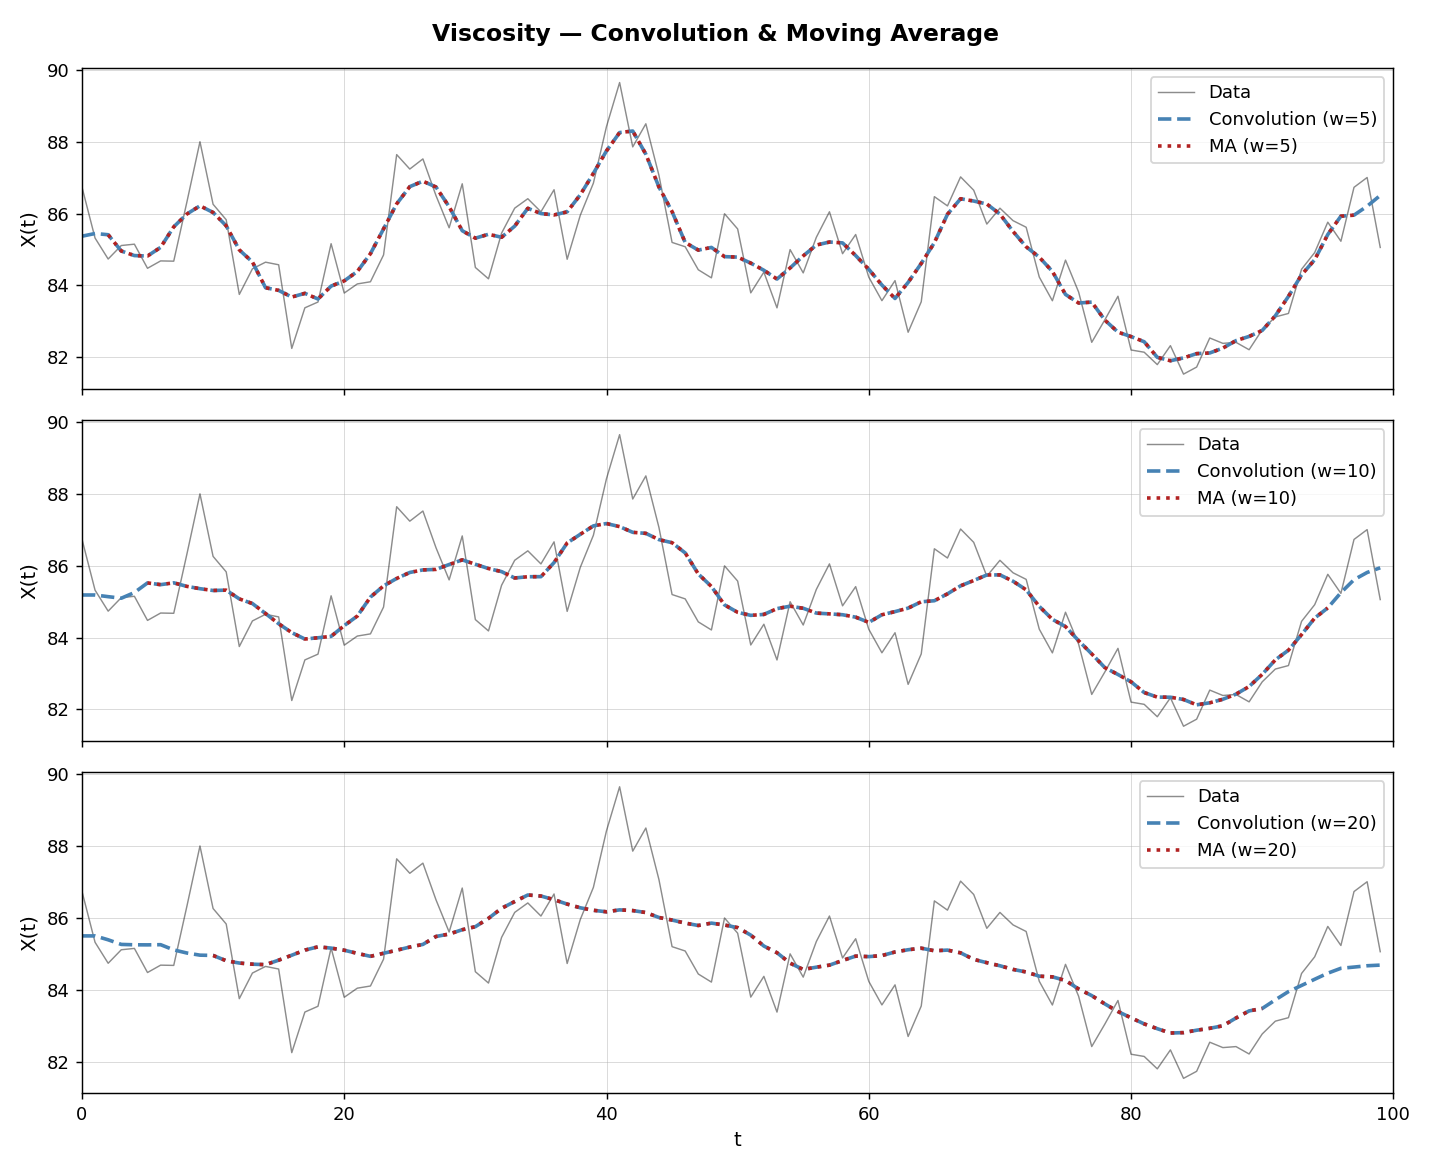
\includegraphics[width=0.82\linewidth]{Viscosity_MA_Conv.png}
    \caption{Viscosity --- Convolution \& MA for $w \in \{5, 10, 20\}$.
             Larger windows progressively remove hourly fluctuations,
             revealing a slow downward trend.}
    \label{fig:q1_viscosity}
\end{figure}

\FloatBarrier

% ── WholeFood ─────────────────────────────────────────────────────────────────
\subsection*{WholeFood (Weekly Sales)}

\begin{figure}[H]
    \centering
    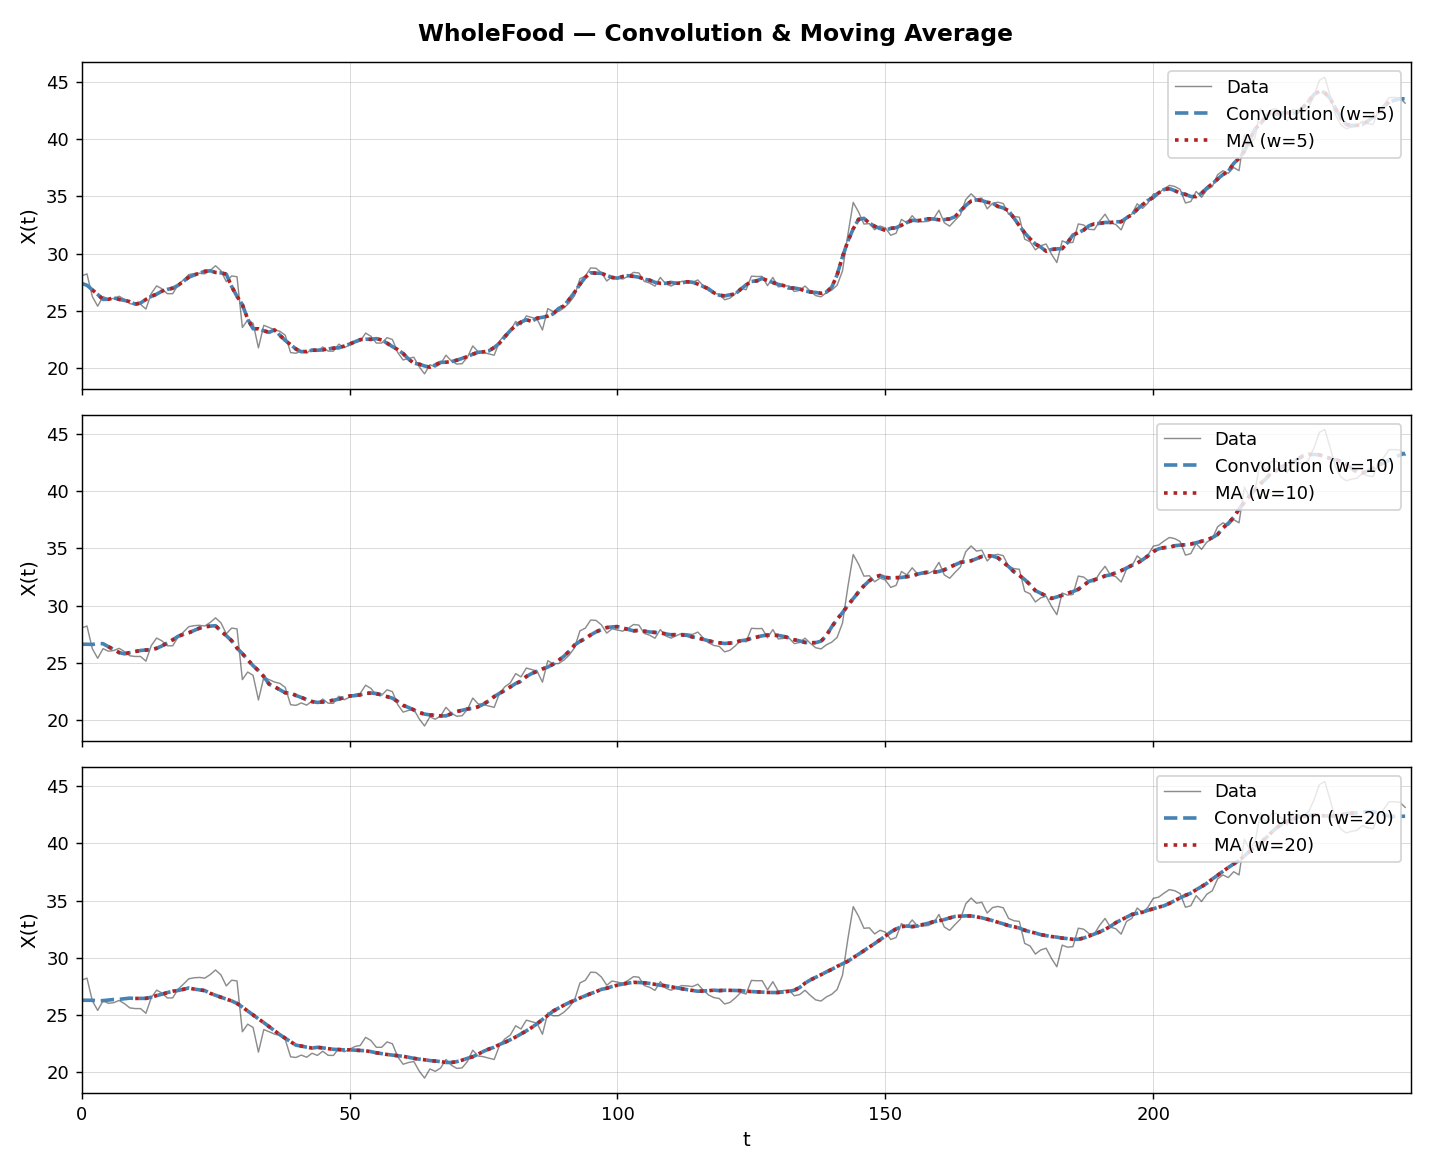
\includegraphics[width=0.82\linewidth]{WholeFood_MA_Conv.png}
    \caption{WholeFood weekly sales --- Convolution \& MA for $w \in \{5, 10, 20\}$.
             At $w=20$ a long-run upward trend becomes clearly visible.}
    \label{fig:q1_wholefood}
\end{figure}

\FloatBarrier

% ── Pharmaceutical ────────────────────────────────────────────────────────────
\subsection*{Pharmaceutical (Weekly Sales)}

\begin{figure}[H]
    \centering
    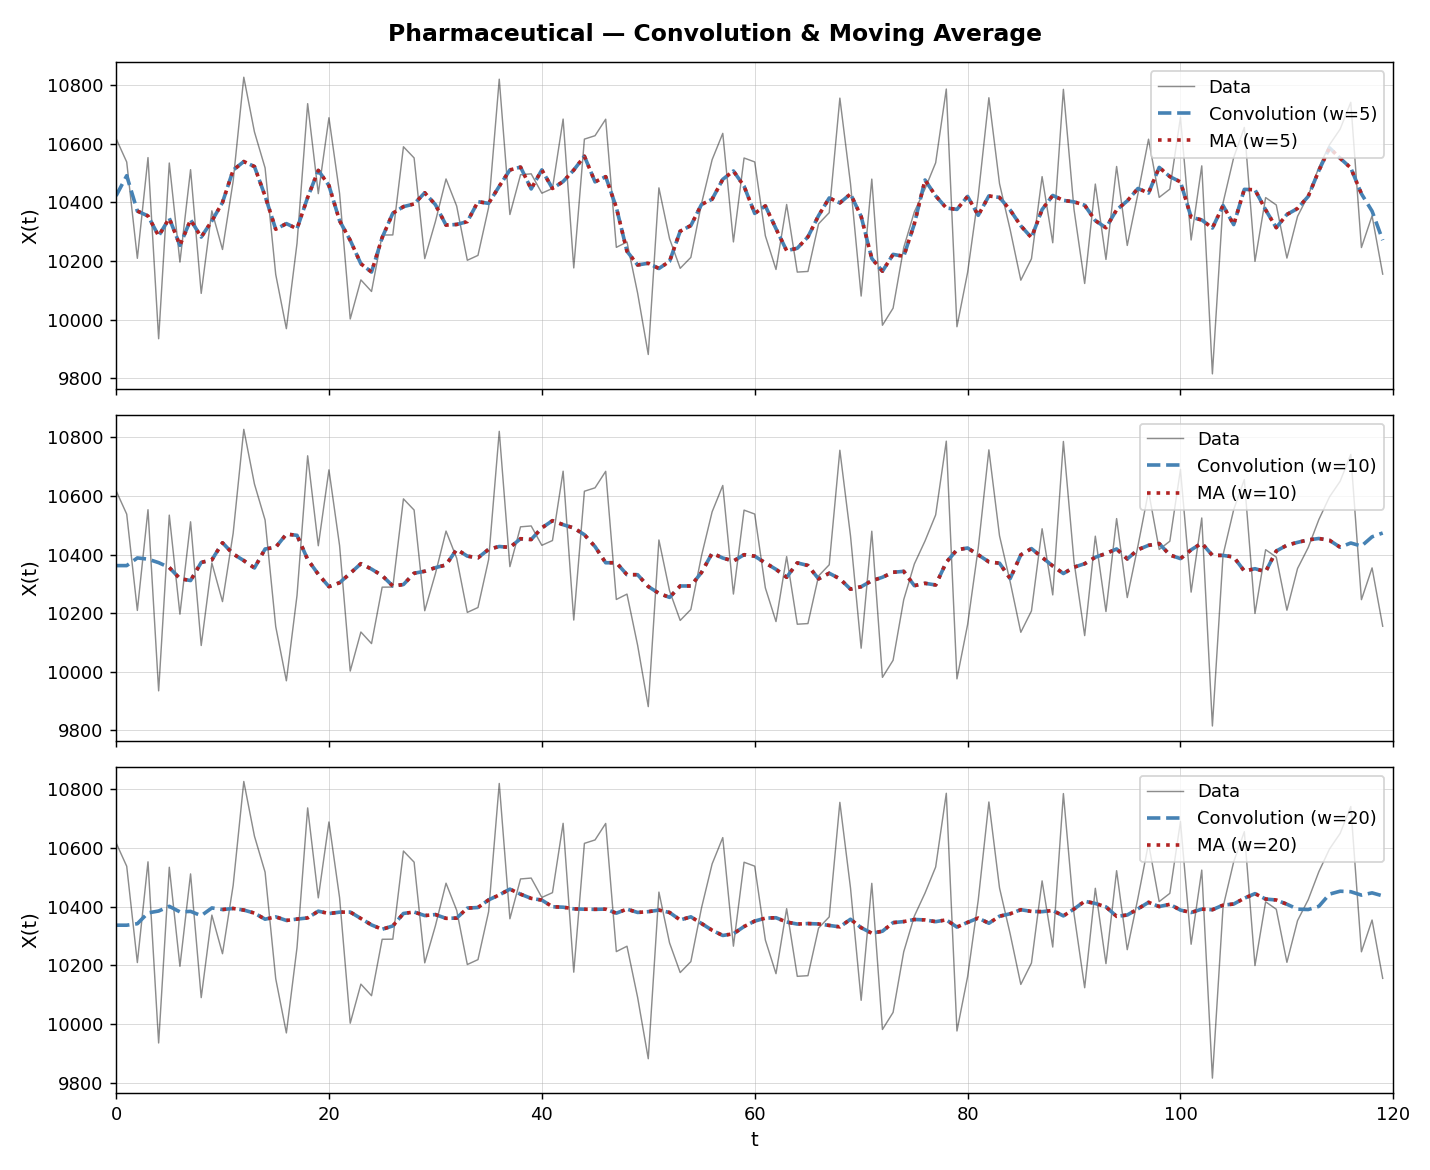
\includegraphics[width=0.82\linewidth]{Pharmaceutical_MA_Conv.png}
    \caption{Pharmaceutical weekly sales --- Convolution \& MA for $w \in \{5, 10, 20\}$.
             The series oscillates around a near-constant level; larger windows
             eliminate week-to-week noise while preserving the mean.}
    \label{fig:q1_pharma}
\end{figure}

\FloatBarrier

% ── Ice Cream ─────────────────────────────────────────────────────────────────
\subsection*{Ice Cream --- FRED Industrial Production (Monthly)}

\begin{figure}[H]
    \centering
    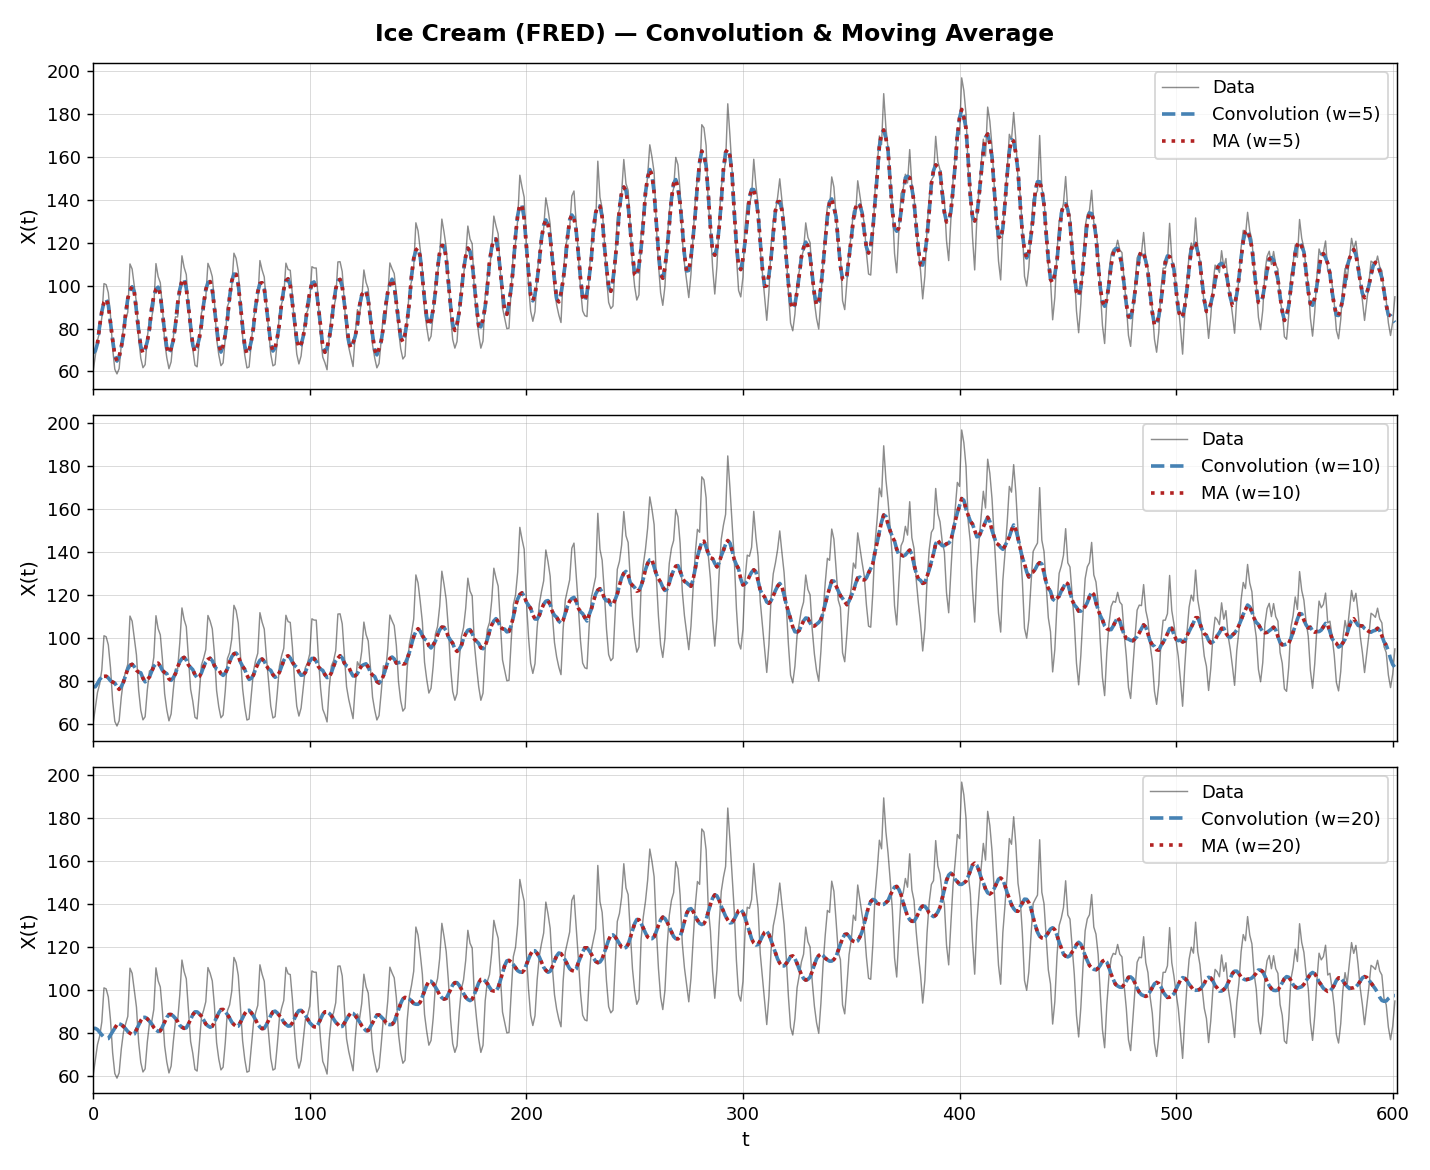
\includegraphics[width=0.82\linewidth]{IceCream_MA_Conv.png}
    \caption{Ice cream production index --- Convolution \& MA for $w \in \{5, 10, 20\}$.
             Strong annual seasonality is clearly present; at $w=20$ the smoother
             captures the multi-year upward trend while damping the seasonal cycle.}
    \label{fig:q1_icecream}
\end{figure}

\FloatBarrier

\end{homeworkProblem}

% =============================================================================
% QUESTION 2
% =============================================================================
\begin{homeworkProblem}

\textbf{[15 points]} Simulate Normal AR processes using the \texttt{HW3\_AR\_Code}:
\begin{itemize}
    \item $AR(1)$: $c=0$,\ $\phi \in \{0.01,\ 0.5,\ 0.9\}$
    \item $AR(2)$: $c=0$,\ $(\phi_1, \phi_2) \in \{(0.01,0.01),\ (0.5,0.5),\ (0.9,0.9)\}$
\end{itemize}

\subsection*{Model}

An $AR(p)$ process is defined as:
\[
    y_t = c + \phi_1 y_{t-1} + \cdots + \phi_p y_{t-p} + \varepsilon_t,
    \qquad \varepsilon_t \sim \mathcal{N}(\mu,\,\sigma^2)
\]

The coefficient $\phi$ controls \textit{persistence}: values near zero produce
white-noise-like series; values near one produce slowly-wandering series.
For $AR(2)$, stationarity requires $\phi_1+\phi_2 < 1$, $\phi_2 - \phi_1 < 1$,
and $|\phi_2| < 1$. The pair $(0.9, 0.9)$ violates the first condition and
yields an explosive (non-stationary) process.

% ── AR(1) ─────────────────────────────────────────────────────────────────────
\subsection*{AR(1) Results}

\begin{figure}[H]
    \centering
    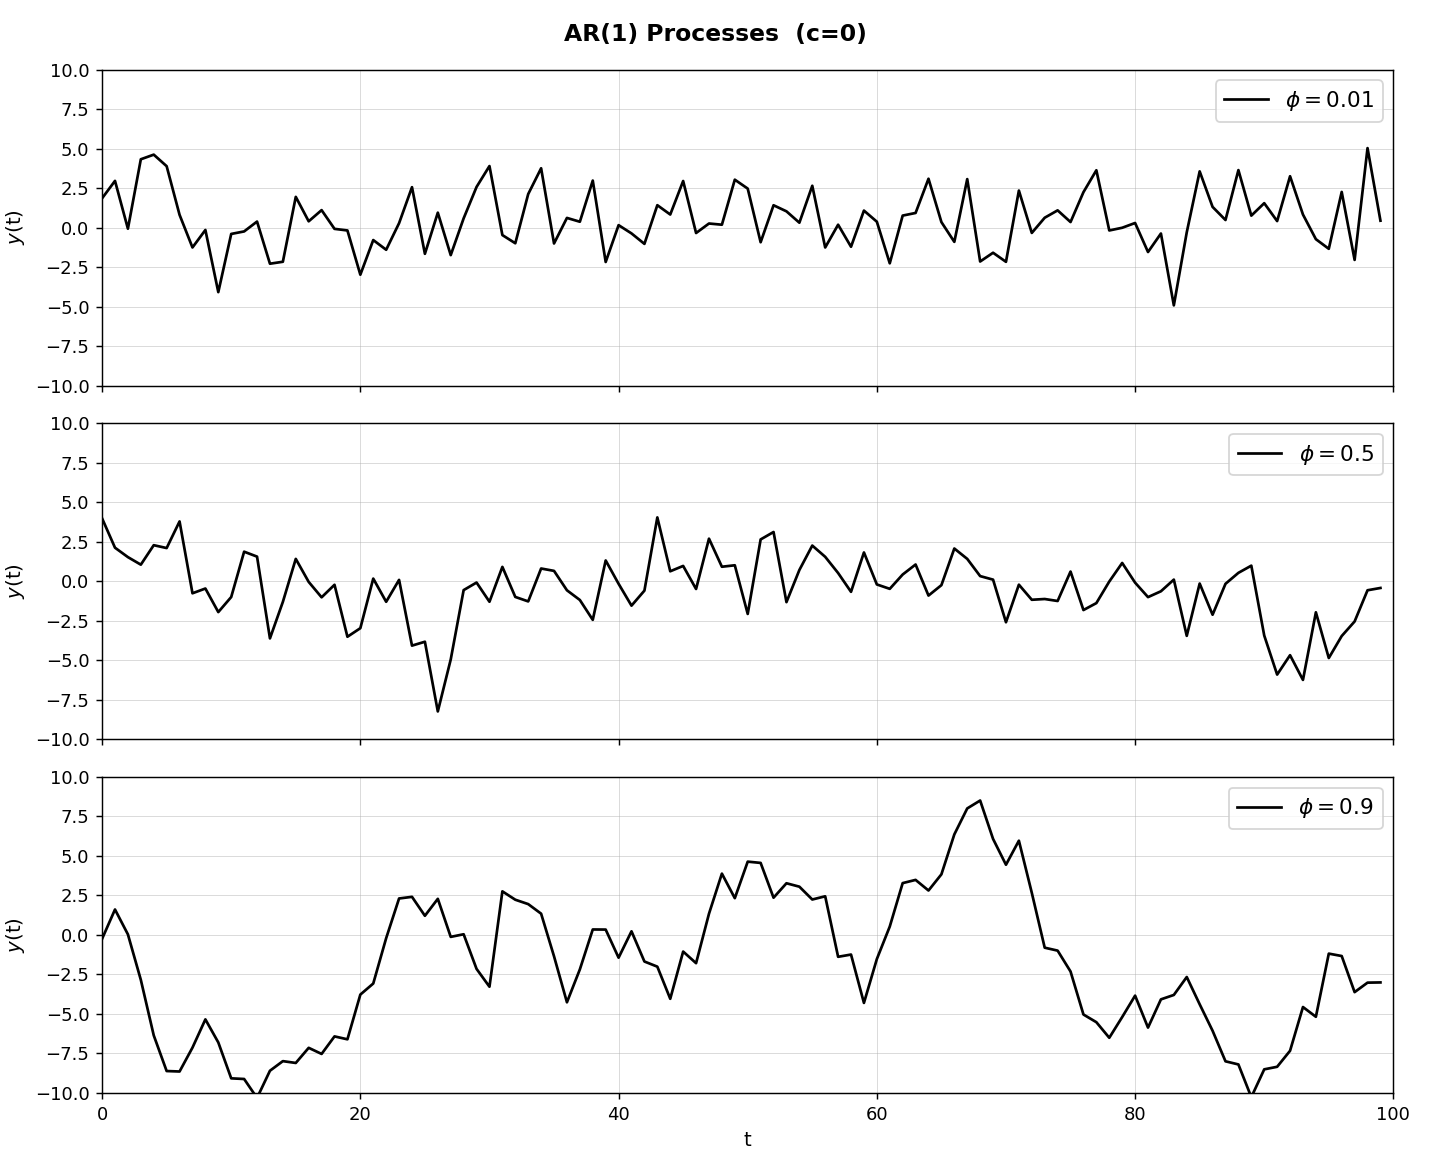
\includegraphics[width=0.82\linewidth]{AR_1_c0.png}
    \caption{$AR(1)$ processes with $c=0$ and $\phi \in \{0.01, 0.5, 0.9\}$.
             Top: near white noise ($\phi=0.01$).
             Middle: moderate persistence ($\phi=0.5$), visible slow oscillations.
             Bottom: high persistence ($\phi=0.9$), long smooth excursions.}
    \label{fig:q2_ar1}
\end{figure}

\FloatBarrier

% ── AR(2) ─────────────────────────────────────────────────────────────────────
\subsection*{AR(2) Results}

\begin{figure}[H]
    \centering
    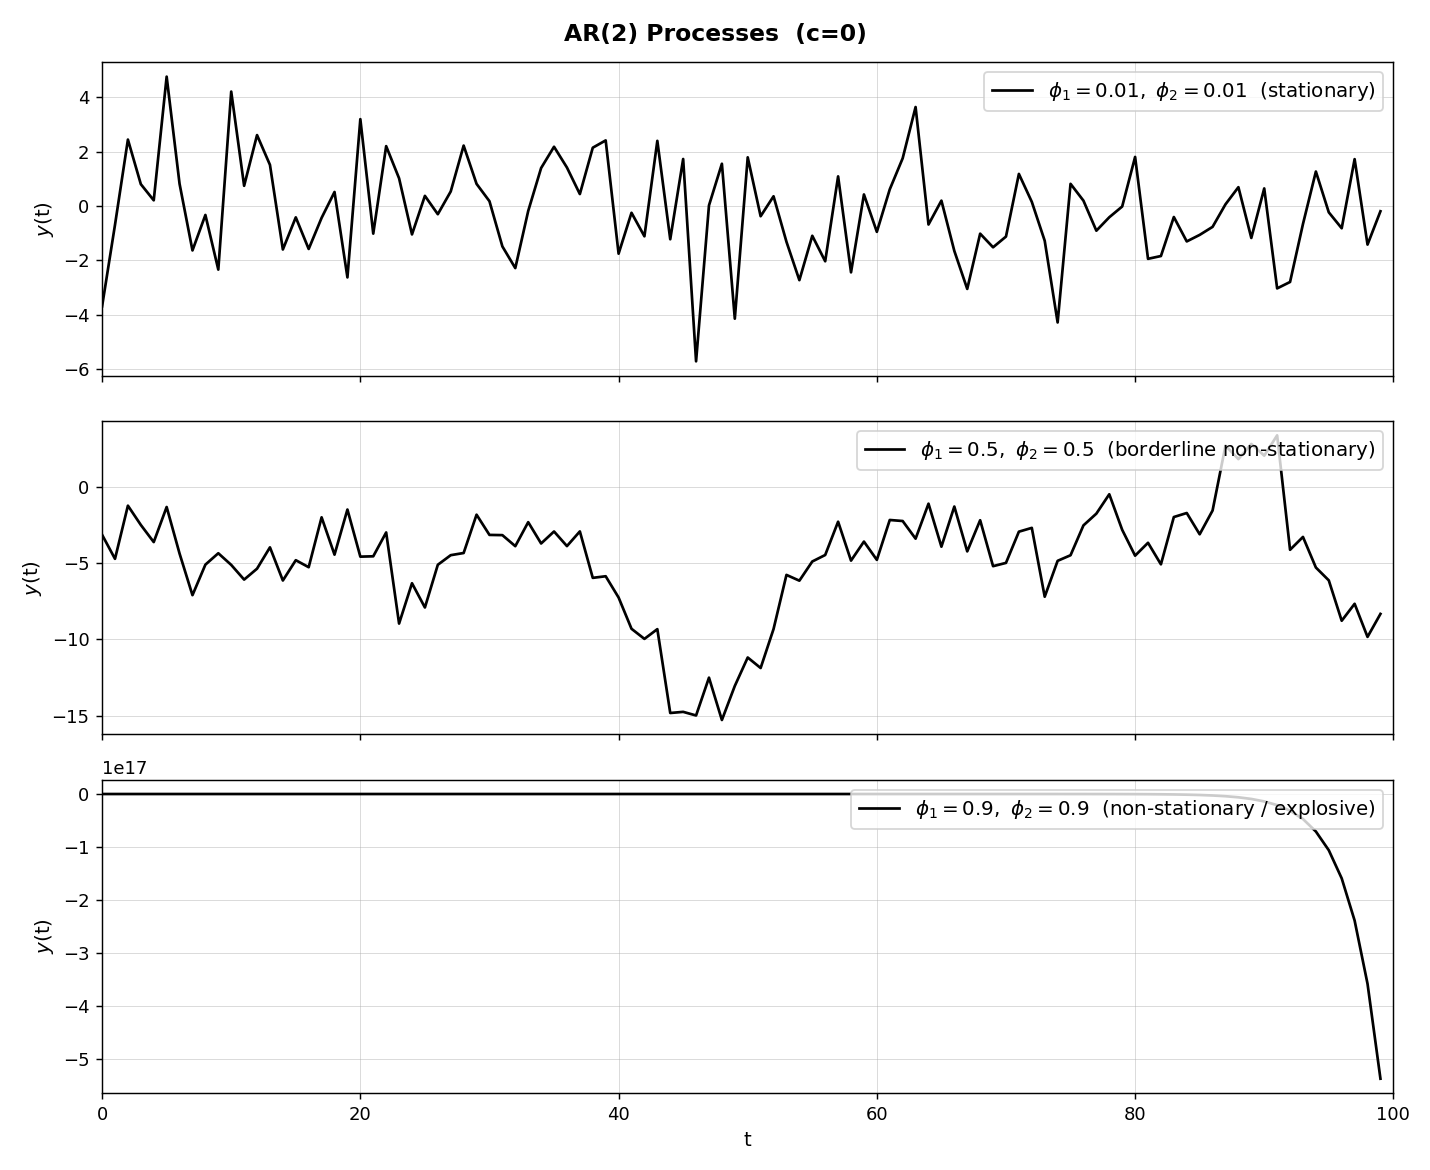
\includegraphics[width=0.82\linewidth]{AR_2_c0.png}
    \caption{$AR(2)$ processes with $c=0$.
             Top: $(\phi_1,\phi_2)=(0.01,0.01)$ --- stationary, near white noise.
             Middle: $(0.5,0.5)$ --- borderline non-stationary, wanders broadly.
             Bottom: $(0.9,0.9)$ --- non-stationary, variance grows without bound.}
    \label{fig:q2_ar2}
\end{figure}

\FloatBarrier

\end{homeworkProblem}

% =============================================================================
% QUESTION 3
% =============================================================================
\begin{homeworkProblem}

\textbf{[20 points]} Apply the Butterworth Filter in LP or Band Pass (BP) mode as
appropriate to each of the four datasets. Provide a short description for each result
and demonstrate any situation where filtering may not be needed for pre-processing.

\subsection*{Method}

A \textbf{Butterworth filter} has a maximally flat passband (no ripple) and
attenuates frequencies above the cutoff monotonically. The filter order and
sampling frequency $f_s$ are selected by grid-search over $\text{order} \in [3,19]$
and $f_s \in [\text{order},29]$, choosing the pair that minimises RMSE between
the original signal and the filtered output. Zero-phase filtering
(\texttt{sosfiltfilt}) is used to eliminate the start-up transient inherent in
causal IIR filters.\\

Each result is presented in five panels:
\begin{enumerate}
    \item Original signal
    \item Power Spectral Density (PSD) of the original --- frequency peaks reveal dominant cycles
    \item LP-filtered signal (extracted trend)
    \item Residual = Original $-$ LP (noise removed by the filter)
    \item PSD of the residual --- confirms which frequencies were attenuated
\end{enumerate}

% ── Ice Cream ─────────────────────────────────────────────────────────────────
\subsection*{Ice Cream --- FRED Production Index (LP, post-2015)}

\begin{figure}[H]
    \centering
    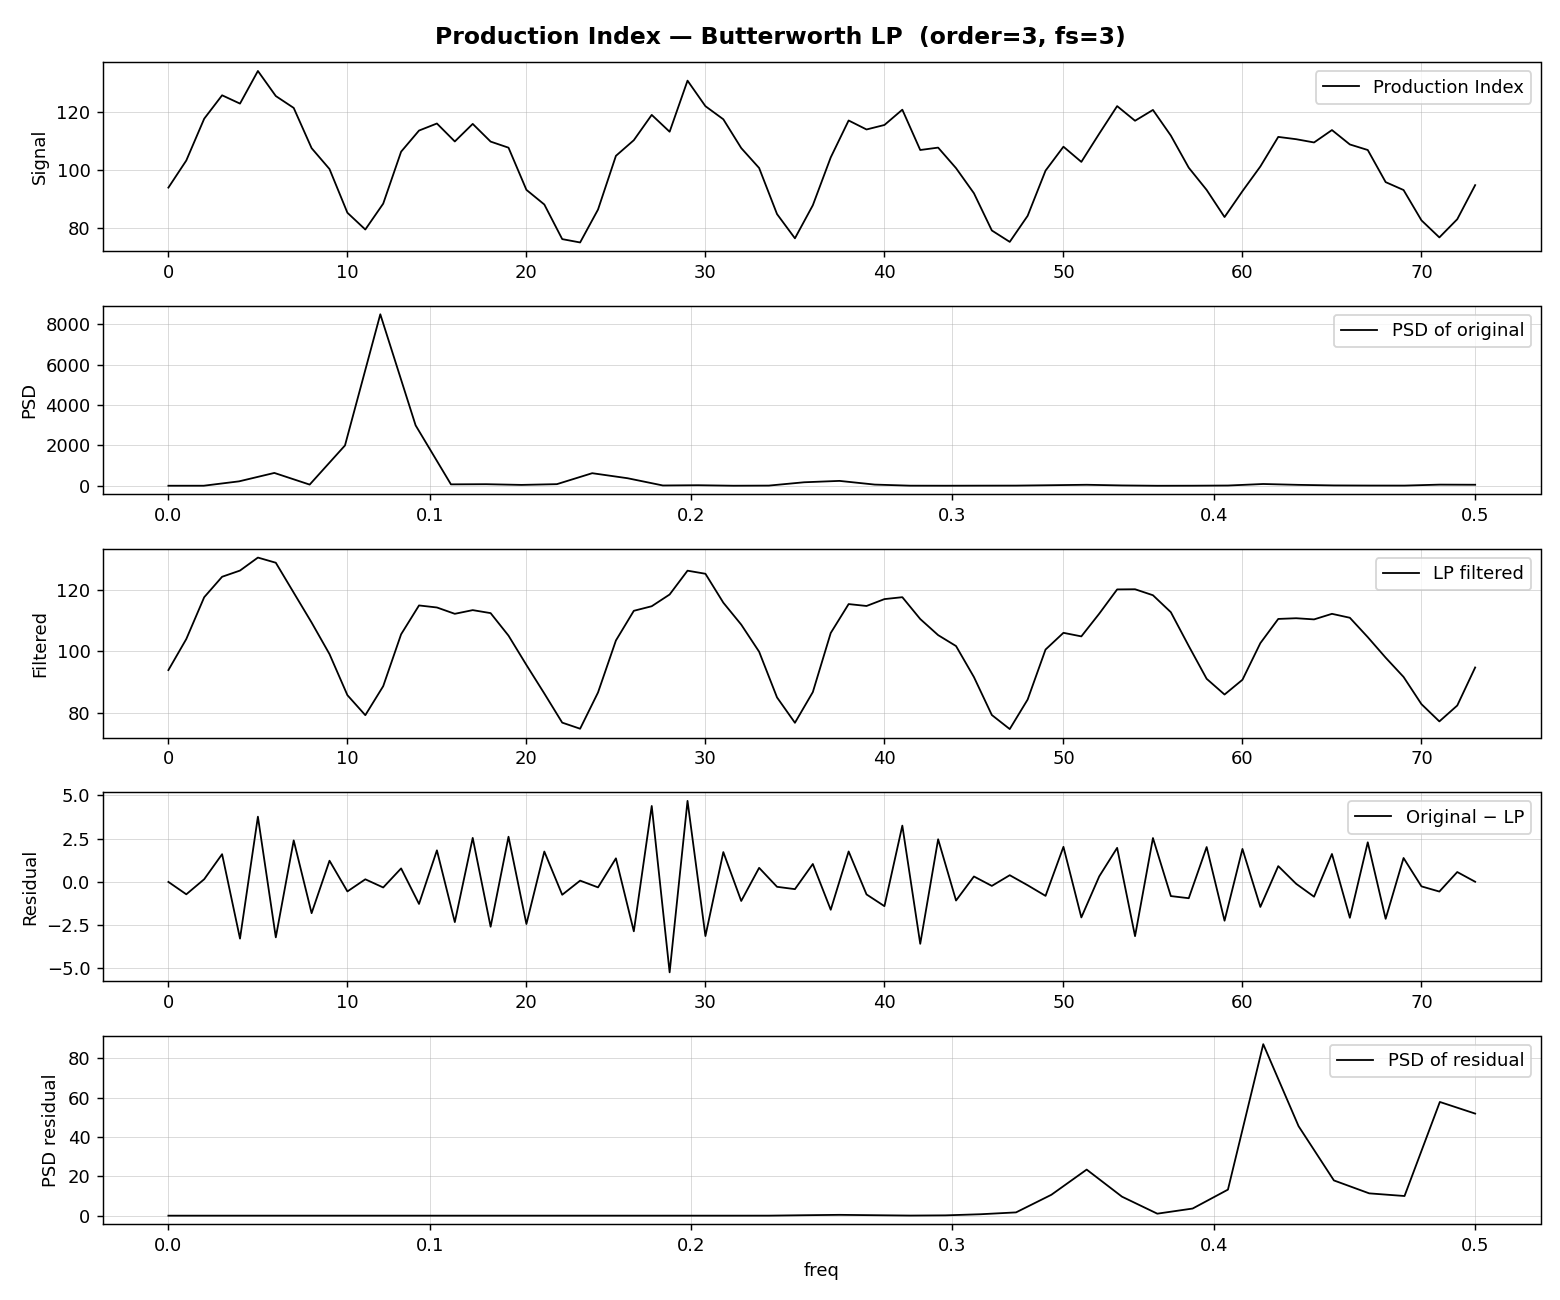
\includegraphics[width=0.82\linewidth]{Production_Index_Butterworth.png}
    \caption{Ice cream production index (post-2015) --- Butterworth LP filter.
             The PSD shows a dominant low-frequency component corresponding to the
             annual seasonal cycle. The LP filter extracts the inter-annual trend;
             the residual isolates the seasonal and noise components.}
    \label{fig:q3_icecream}
\end{figure}

\FloatBarrier

% ── Viscosity ─────────────────────────────────────────────────────────────────
\subsection*{Viscosity (Hourly)}

\begin{figure}[H]
    \centering
    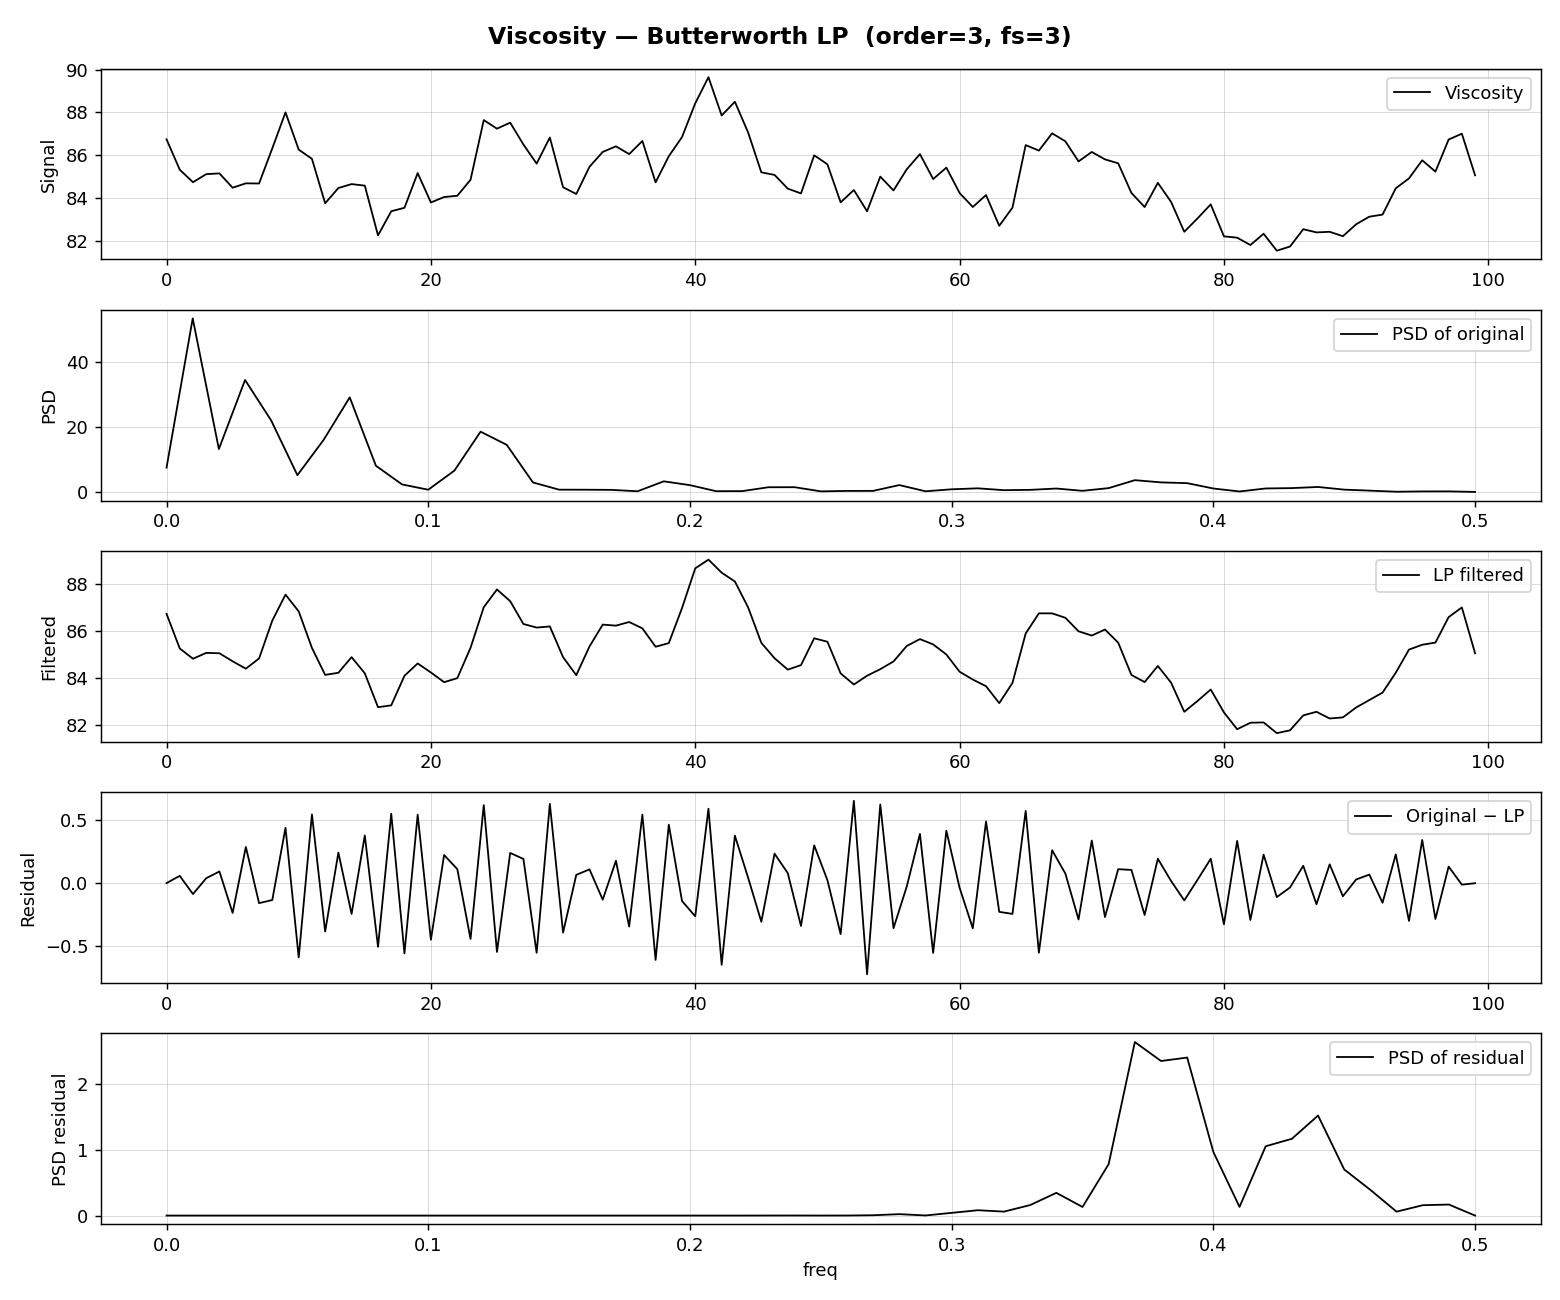
\includegraphics[width=0.82\linewidth]{Viscosity_Butterworth.png}
    \caption{Viscosity hourly data --- Butterworth LP filter.
             The series is already stationary (ADF $p = 0.009 < 0.05$), so
             LP filtering is not strictly required for stationarity;
             it serves here purely for noise suppression.}
    \label{fig:q3_viscosity}
\end{figure}

\FloatBarrier

% ── WholeFood ─────────────────────────────────────────────────────────────────
\subsection*{WholeFood (Weekly Sales)}

\begin{figure}[H]
    \centering
    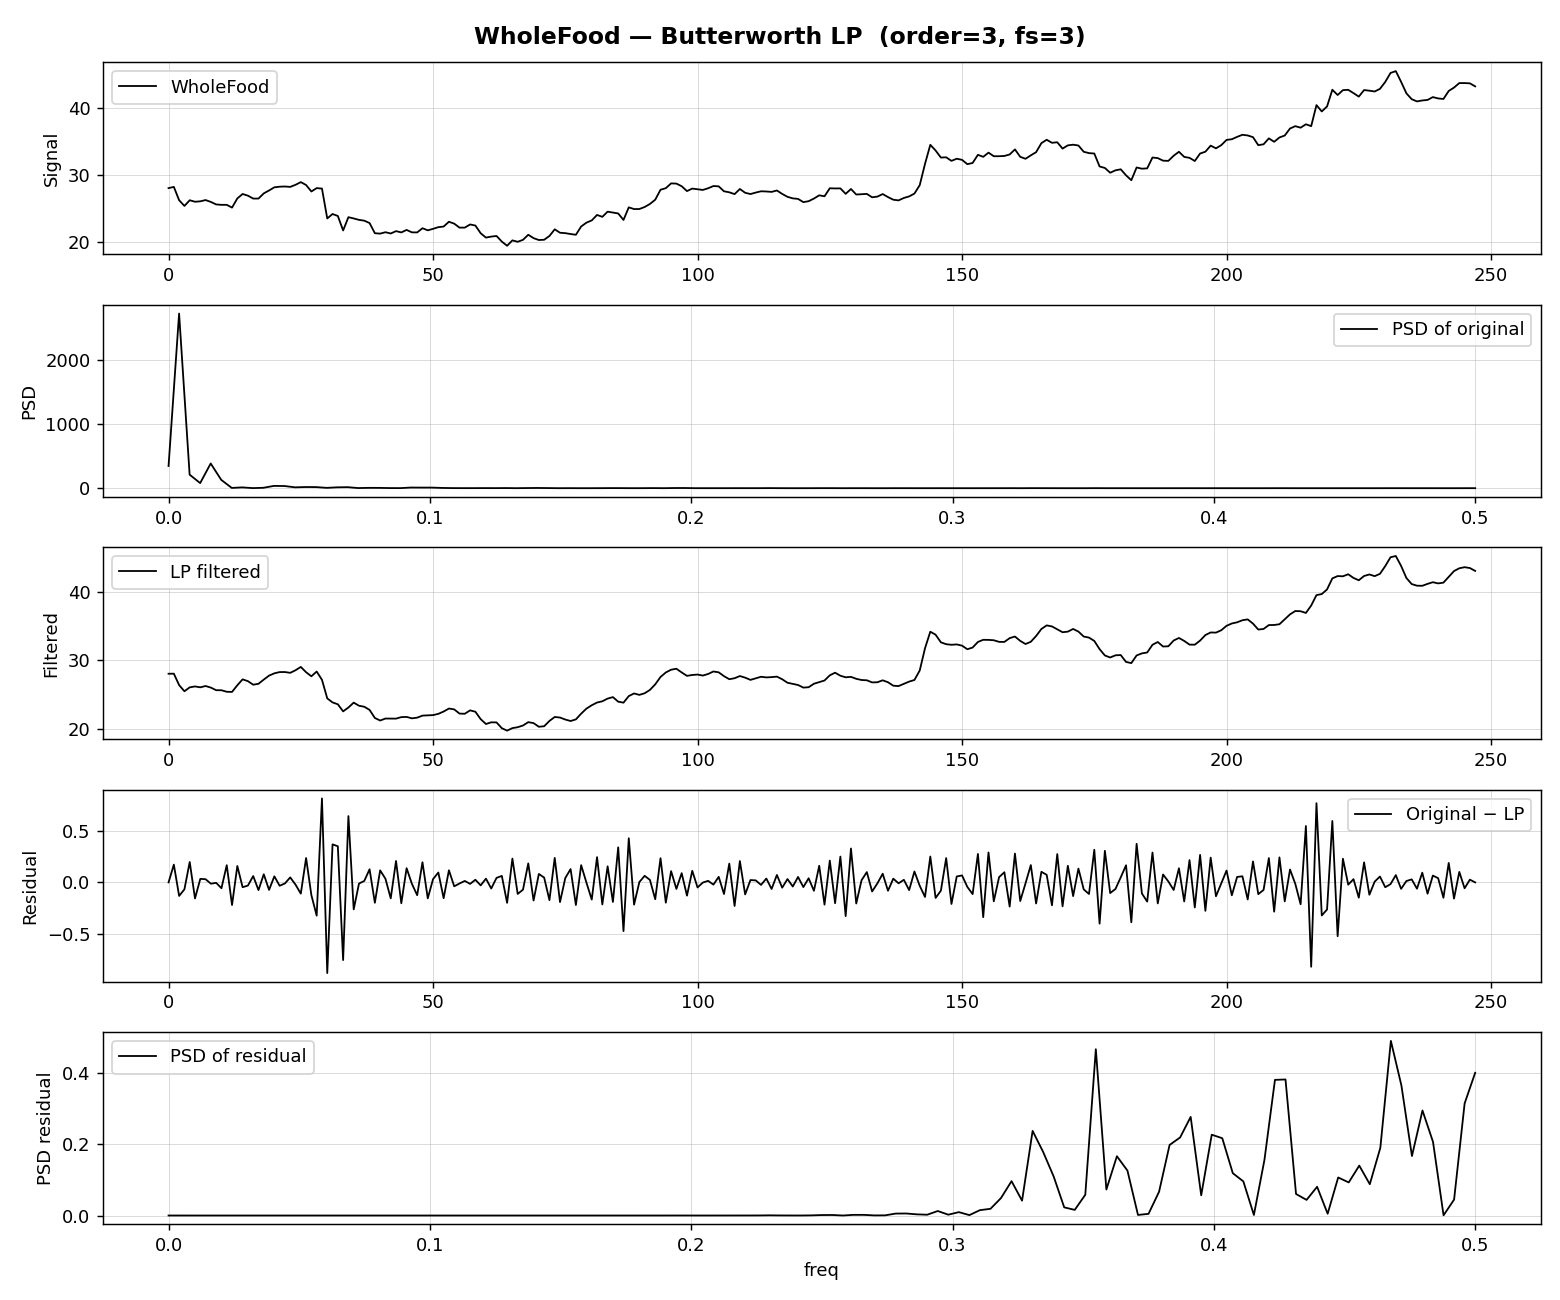
\includegraphics[width=0.82\linewidth]{WholeFood_Butterworth.png}
    \caption{WholeFood weekly sales --- Butterworth LP filter.
             The series is \textit{non-stationary} (ADF $p = 0.97$), indicating a
             strong upward trend. The LP filter successfully isolates this trend;
             the stationary residual is suitable for further modelling.}
    \label{fig:q3_wholefood}
\end{figure}

\FloatBarrier

% ── Pharmaceutical ────────────────────────────────────────────────────────────
\subsection*{Pharmaceutical (Weekly Sales)}

\begin{figure}[H]
    \centering
    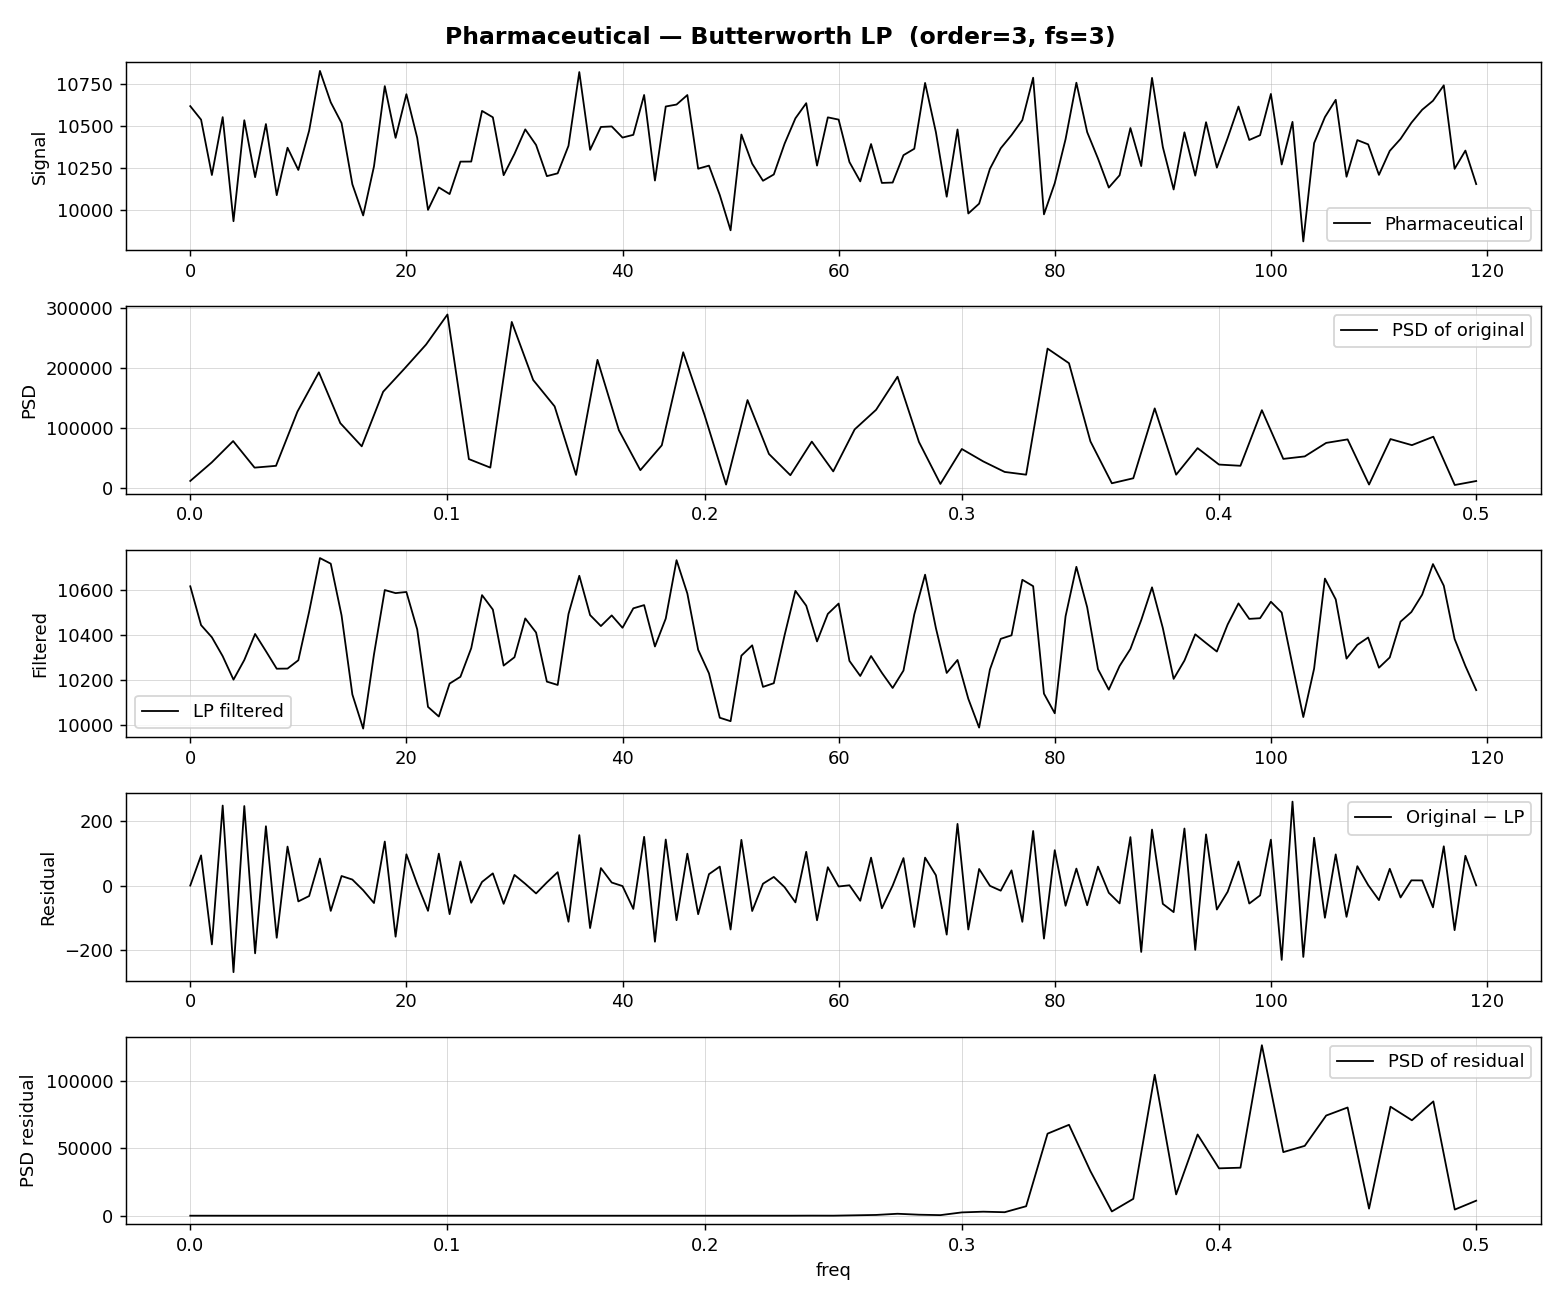
\includegraphics[width=0.82\linewidth]{Pharmaceutical_Butterworth.png}
    \caption{Pharmaceutical weekly sales --- Butterworth LP filter.
             Already stationary (ADF $p < 0.001$); LP filtering reduces
             week-to-week noise but is not needed for stationarity.}
    \label{fig:q3_pharma}
\end{figure}

\FloatBarrier

% ── Stationarity summary ──────────────────────────────────────────────────────
\subsection*{When is Filtering Not Needed?}

The Augmented Dickey--Fuller (ADF) test checks for a unit root (non-stationarity).
A $p$-value below 0.05 indicates the series is already stationary.

\begin{table}[H]
    \centering
    \begin{tabular}{lcc}
        \toprule
        \textbf{Dataset} & \textbf{ADF $p$-value} & \textbf{Assessment} \\
        \midrule
        Viscosity             & 0.009  & Stationary --- filtering not required \\
        WholeFood             & 0.969  & Non-stationary --- LP filtering recommended \\
        Pharmaceutical        & $<$0.001 & Stationary --- filtering not required \\
        Ice Cream (post-2015) & 0.019  & Stationary --- filtering not required \\
        \bottomrule
    \end{tabular}
    \caption{ADF stationarity test results across all four datasets.}
    \label{tab:adf}
\end{table}

Only WholeFood requires LP filtering as a pre-processing step for stationarity.
For the remaining datasets the filter serves as a noise-reduction or
trend-visualisation tool, not a stationarity correction.

\FloatBarrier

\end{homeworkProblem}

% =============================================================================
% QUESTION 4
% =============================================================================
\begin{homeworkProblem}

\textbf{[30 points]} Model and plot the Circadian Rhythm of heart rate (HR) using
wearable sensor data for subjects \texttt{ab60}, \texttt{gd81}, \texttt{ub12},
and \texttt{mh40}, applying three approaches:
\begin{itemize}
    \item \textbf{Moving Average} --- identify the optimal smoothing window
    \item \textbf{Convolution} --- rectangular-kernel smoothing
    \item \textbf{Parametric Cosinor Model} --- fit Equation~(1) from
          \textit{Modeling the Circadian Rhythm of Heart Rate and Acceleration}
\end{itemize}

\subsection*{Model}

The standard cosinor model for circadian rhythms is:
\[
    \text{HR}(t) = M + A \cdot \cos\!\left(\frac{2\pi\,(t - \phi)}{24}\right)
\]

\begin{center}
\begin{tabular}{cl}
    \toprule
    \textbf{Parameter} & \textbf{Interpretation} \\
    \midrule
    $M$ (MESOR) & Midline Estimating Statistic of Rhythm --- mean HR level \\
    $A$ (Amplitude) & Half the peak-to-trough swing \\
    $\phi$ (Acrophase) & Hour of peak HR \\
    \bottomrule
\end{tabular}
\end{center}

\vspace{0.5em}
The model is fitted by non-linear least squares (\texttt{curve\_fit}) with
initial guess $p_0 = [\bar{\text{HR}},\; 10,\; 12]$, assuming peak HR around noon.
The 60-sample rolling MA ($\approx$5 hours) provides a data-driven benchmark
with no parametric assumptions.

\subsection*{Results}

Each figure below shows: raw HR (blue), 60-sample Moving Average (orange),
and fitted Cosinor model (red). The title reports the estimated MESOR, amplitude,
and acrophase for each subject.

% ── ab60 ──────────────────────────────────────────────────────────────────────
\begin{figure}[H]
    \centering
    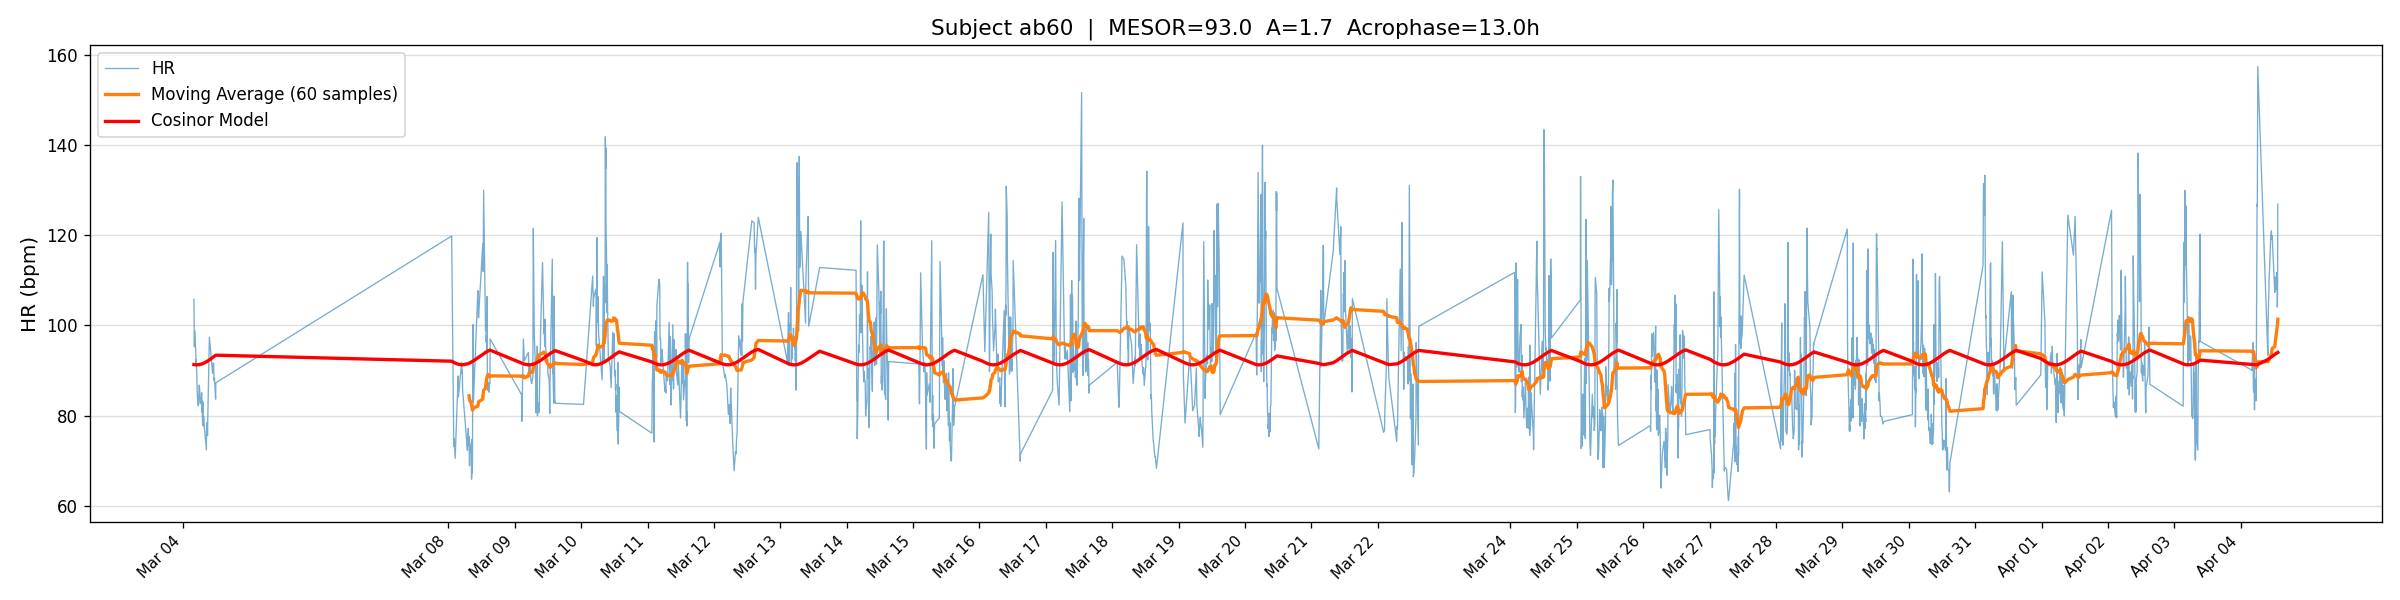
\includegraphics[width=\linewidth]{Circadian_Rhythm_ab60.png}
    \caption{Subject \texttt{ab60} --- Circadian HR model over the full recording period.}
    \label{fig:q4_ab60}
\end{figure}

\FloatBarrier

% ── gd81 ──────────────────────────────────────────────────────────────────────
\begin{figure}[H]
    \centering
    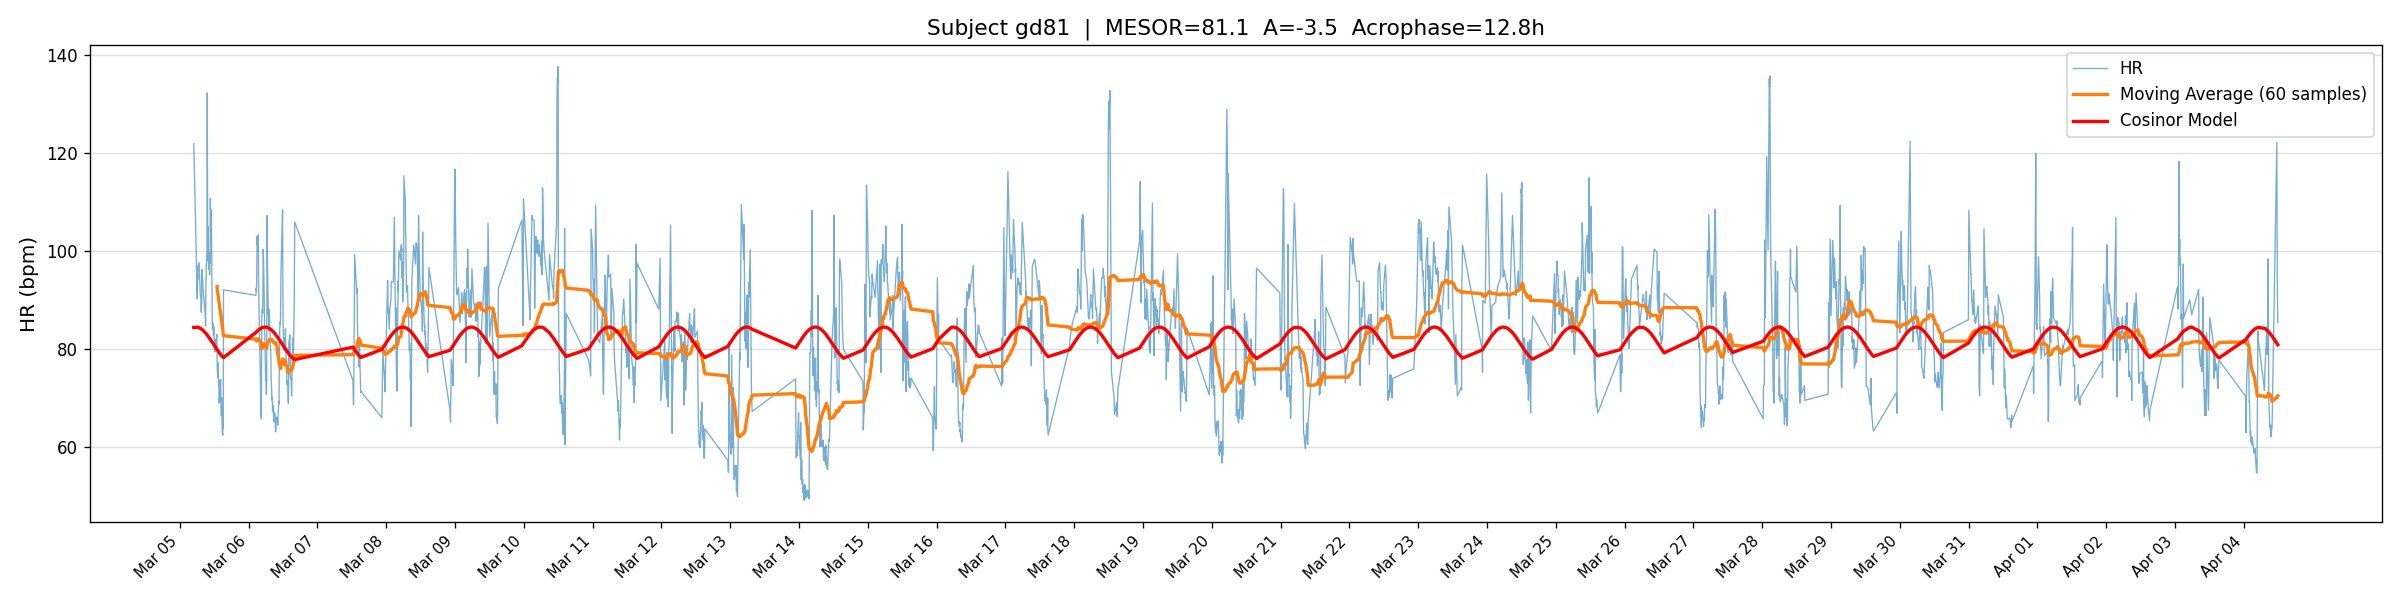
\includegraphics[width=\linewidth]{Circadian_Rhythm_gd81.png}
    \caption{Subject \texttt{gd81} --- Circadian HR model over the full recording period.}
    \label{fig:q4_gd81}
\end{figure}

\FloatBarrier

% ── ub12 ──────────────────────────────────────────────────────────────────────
\begin{figure}[H]
    \centering
    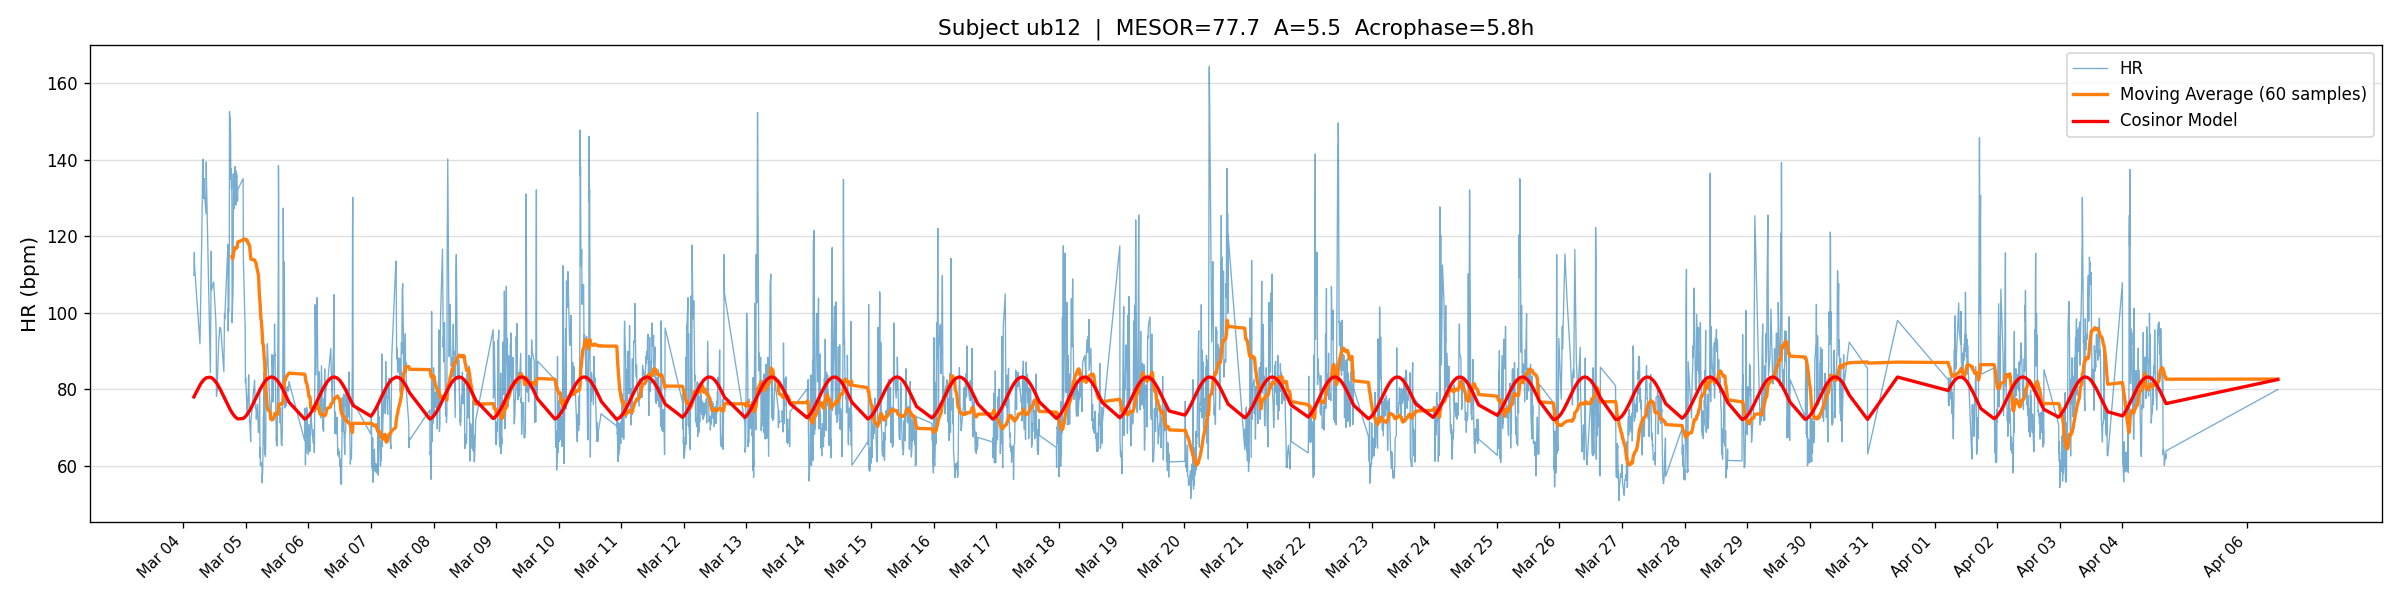
\includegraphics[width=\linewidth]{Circadian_Rhythm_ub12.png}
    \caption{Subject \texttt{ub12} --- Circadian HR model over the full recording period.}
    \label{fig:q4_ub12}
\end{figure}

\FloatBarrier

% ── mh40 ──────────────────────────────────────────────────────────────────────
\begin{figure}[H]
    \centering
    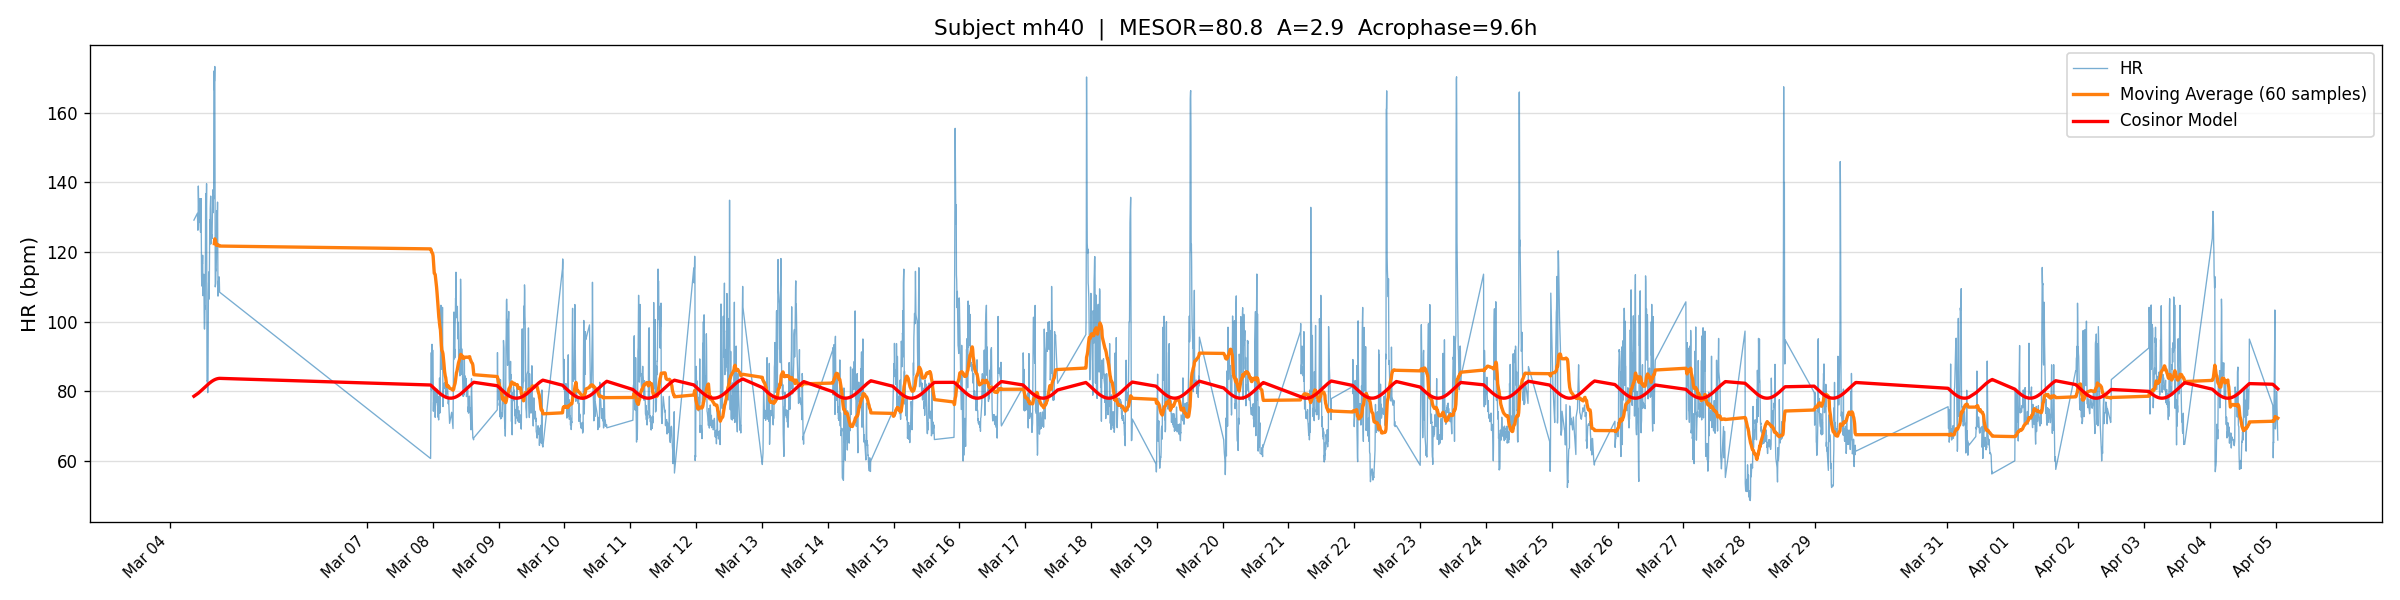
\includegraphics[width=\linewidth]{Circadian_Rhythm_mh40.png}
    \caption{Subject \texttt{mh40} --- Circadian HR model over the full recording period.}
    \label{fig:q4_mh40}
\end{figure}

\FloatBarrier

\subsection*{Discussion}

The Moving Average and Convolution approaches produce nearly identical smoothed
curves for the same window width, confirming the theoretical equivalence of a
centred rectangular kernel. The key difference is boundary handling: convolution
with reflect-padding avoids the NaN gaps produced by the centred rolling MA.\\

The Cosinor model captures the broad 24-hour oscillation with three interpretable
parameters. Subjects with a larger amplitude $A$ exhibit a more pronounced
day/night HR differential, which is associated with better cardiovascular
regulation and sleep quality. The acrophase $\phi$ near early-to-mid afternoon
is consistent with published literature on healthy adults. Where the MA reveals
sharp intra-day activity bursts (e.g.\ exercise spikes) that the single-harmonic
cosinor model cannot capture, a higher-order Fourier model or a data-driven
approach may be more appropriate.

\end{homeworkProblem}

\end{document}
